\section{Experiments and Evaluations}

This section describes in progress and proposed studies to support this thesis. The bracketed text represents short names for each experiment and the text in parentheses displays the status and semester of submission.


%Peer learning is the process of acquiring knowledge and skills through interactions with colleagues. This type of collaboration is also important for increasing learning among software engineers, however it rarely occurs in industry. For example, Murphy-Hill and colleagues found that interactions between developers is the most effective mode of tool discovery, but they also occur infrequently in practice~\cite{Murphy-Hill2011PeerInteraction}. There are many ways for open source software developers to convey information to peers, and this study aims to discover the best way to increase peer learning for GitHub users. This research seeks to gather data describing how developers react to learning about new tools through recommendations from varying systems: emails, project issues\footnote{https://help.github.com/en/articles/about-issues}, pull requests\footnote{https://help.github.com/en/articles/about-pull-requests}, and suggestions\footnote{https://github.blog/changelog/2018-10-16-suggested-changes/}. Then, we conduct an in-depth analysis on the preferred method reported by participants to determine how effective and useful that feature is for learning in practice.

\subsection{[\suggT] ``Understanding the Impact of GitHub \emph{Suggested Changes} on Recommendations Between Developers" (In Submission, Fall 2019)}

\subsubsection{Motivation:} GitHub recently introduced a new feature, \textit{suggested changes},\footnote{\url{https://help.github.com/articles/incorporating-feedback-in-your-pull-request/\#applying-a-suggested-change}} which fosters peer interactions online by allowing developers to recommend code changes to each other during code reviews through this novel system. We chose to analyze this novel feature because it has become very popular on GitHub, with developers ``quick to adopt suggested changes" into their workflow and totaled over 100,000 uses within weeks of the initial release, accounting for approximately 4\% of pull request review comments and 10\% of code  reviewers.\footnote{\label{SuggestBlog}\url{https://github.blog/2018-11-01-suggested-changes-update/}} Additionally, the GitHub suggested changes feature can be considered an example of a digital nudge and adheres to the developer recommendation choice architectures. This research seeks to discover the impact of the recently introduced suggested changes feature by gathering data about the developer usage and effectiveness of these suggestions, collecting feedback from developers about the new feature, and exploring how well the design of this feature generalizes to other types of recommendations. To our knowledge, this is the first study to analyze the suggested changes feature on GitHub. The results from this work provide implications to improve the effectiveness of recommendations to developers and are used to motivate the design of future automated recommender systems.

\subsubsection{Suggested Changes:} GitHub released suggested changes as a public beta feature in October 2018. This new feature to allow GitHub users to recommend code changes on pull requests to software developers. Figures \ref{fig:sugg}a-c present how the suggested changes feature works. When a reviewer notices a line of code that can be improved, they can click on the plus (+) sign on the line of code in question to write a comment and create a suggestion. Then, the text box in Figure \ref{fig:sugg}a pops up for the users to enter their proposed change. Figure \ref{fig:sugg}b shows a developer typing their suggested code change for the pull request into the text box. Once the reviewer is finished with their suggestion, they can click on the ``Start a review" button to submit the suggested change. Finally, the developer who created the pull request can see the suggested change on their code, shown in Figure \ref{fig:sugg}c, and can commit, edit, or ignore the proposed modifications. Clicking ``Commit changes" will automatically add the change to the pull request as a new commit. Suggested changes can be considered a nudge because they are used to encourage developers to improve code in their pull requests without providing incentives for committing suggestions or prohibiting alternative changes to improve the code. Additionally, this feature also implements our developer recommendation choice architectures presented in Section 5: they are \textit{actionable} by allowing developers to immediately apply recommendations by clicking on a button to commit (Figure~\ref{fig:sugg}c); provide specific \textit{feedback} to users by providing an improvement to the code with an optional comment (Figure~\ref{fig:sugg}b); have high \textit{spatial locality} with recommendations appearing to developers on the exact line of code in their pull request; and have convenient \textit{temporal locality} during code reviews before merging the code.

% \begin{figure*}[]
% \subfloat[Reviewer adds comment~]{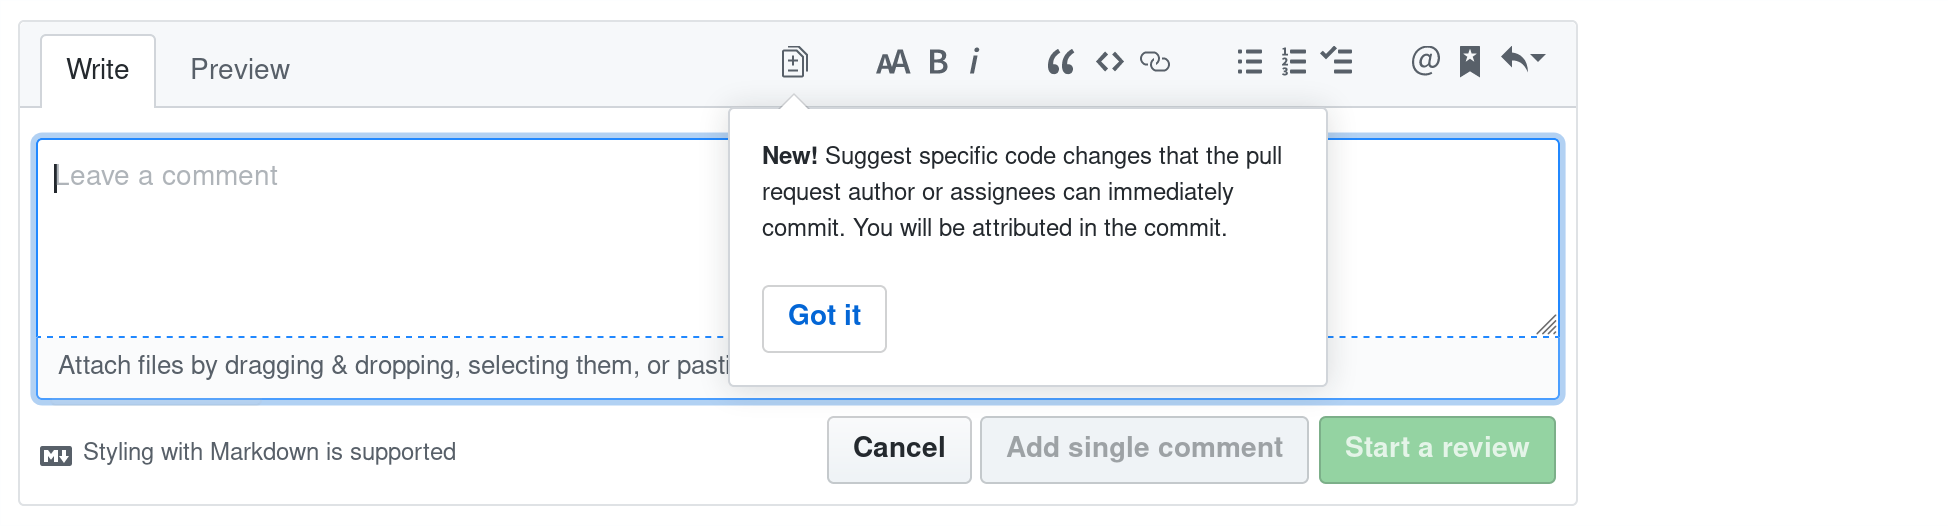
\includegraphics[width=\linewidth]{images/sugg1.png}}
% \subfloat[Reviewer suggests change~]{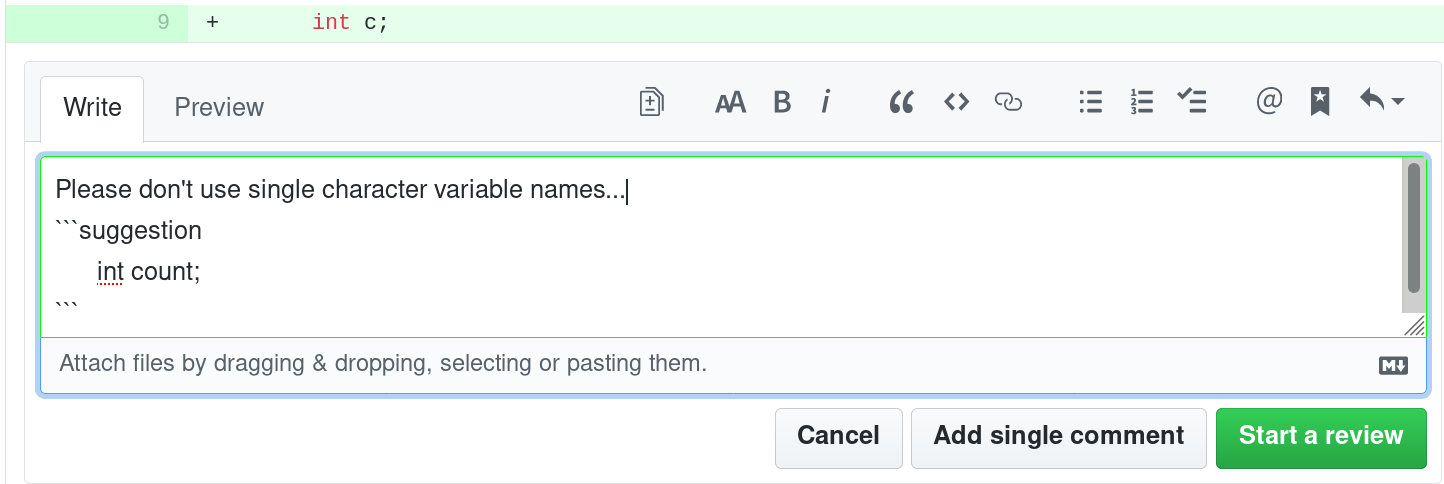
\includegraphics[width=\linewidth]{images/sugg2.png}}
% \subfloat[Developer applies suggestion]{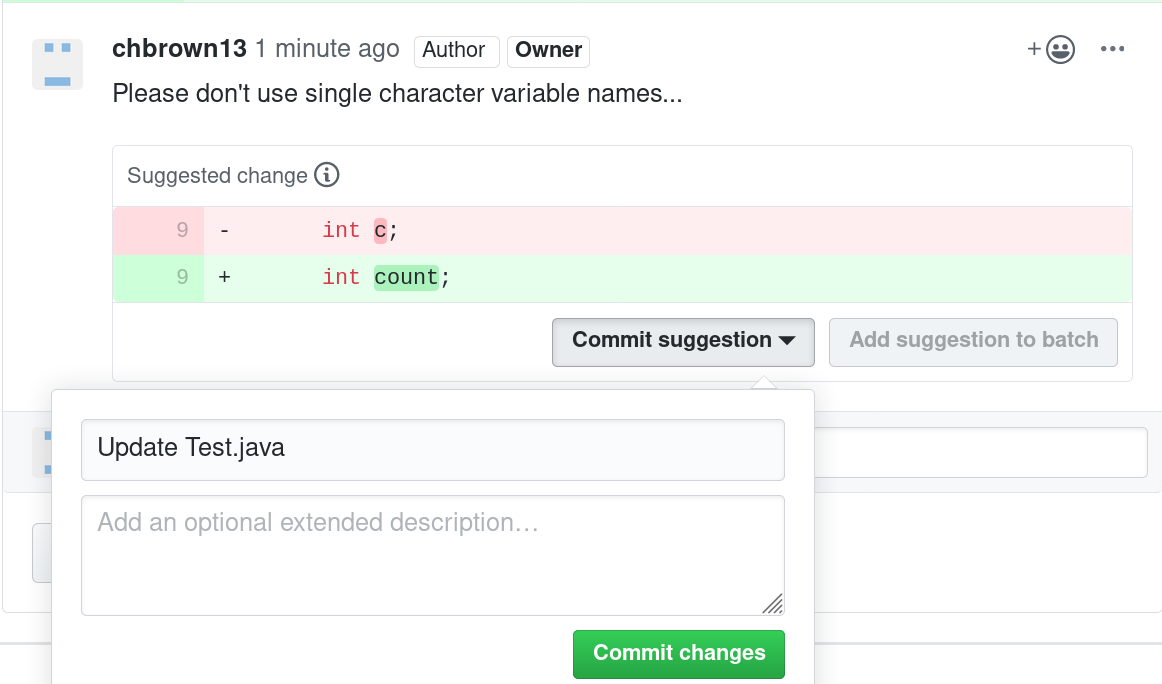
\includegraphics[width=\linewidth]{images/sugg3.png}}
% \caption{GitHub Suggested Changes example}
% \label{fig:sugg}
% \end{figure*}

\begin{figure}[]
\centering
    (a) Reviewer adds a pull request comment \\
    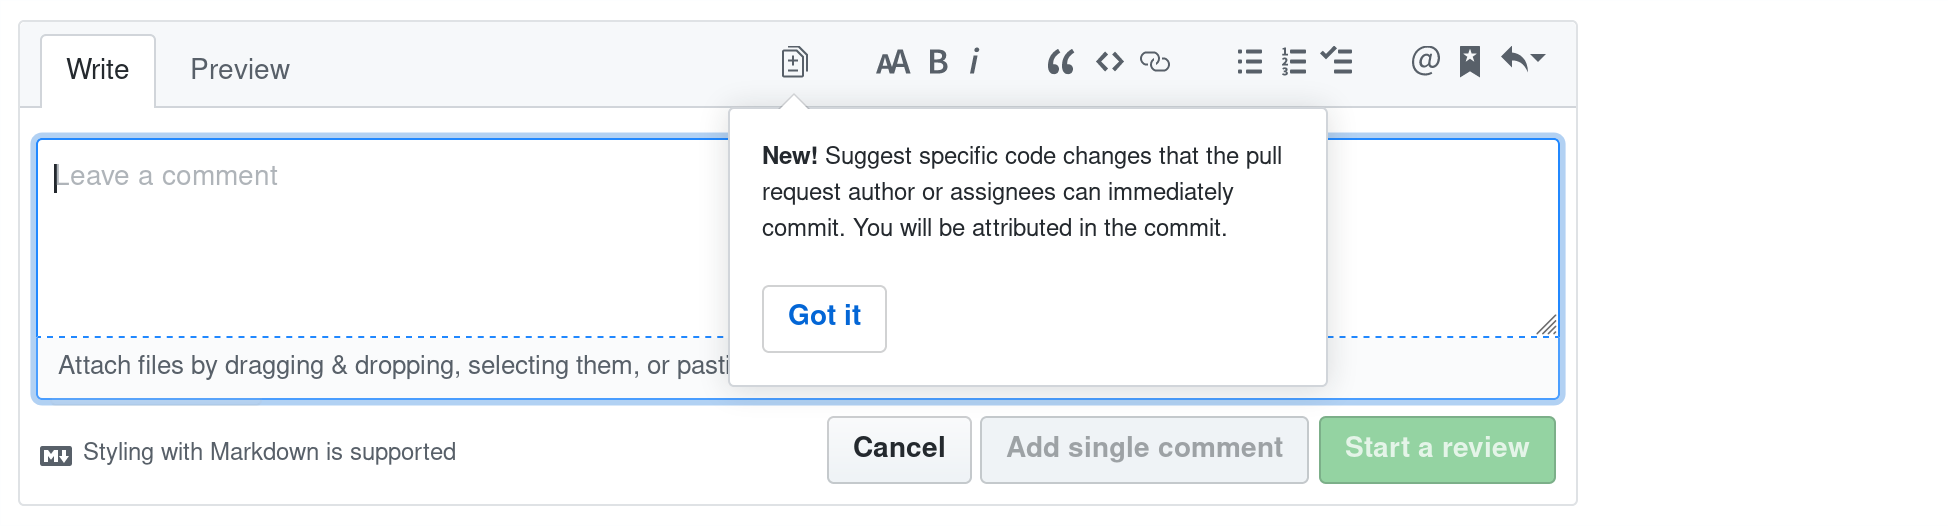
\includegraphics[width=\textwidth]{images/sugg1.png}
    (b) Reviewer suggests a code change \\
    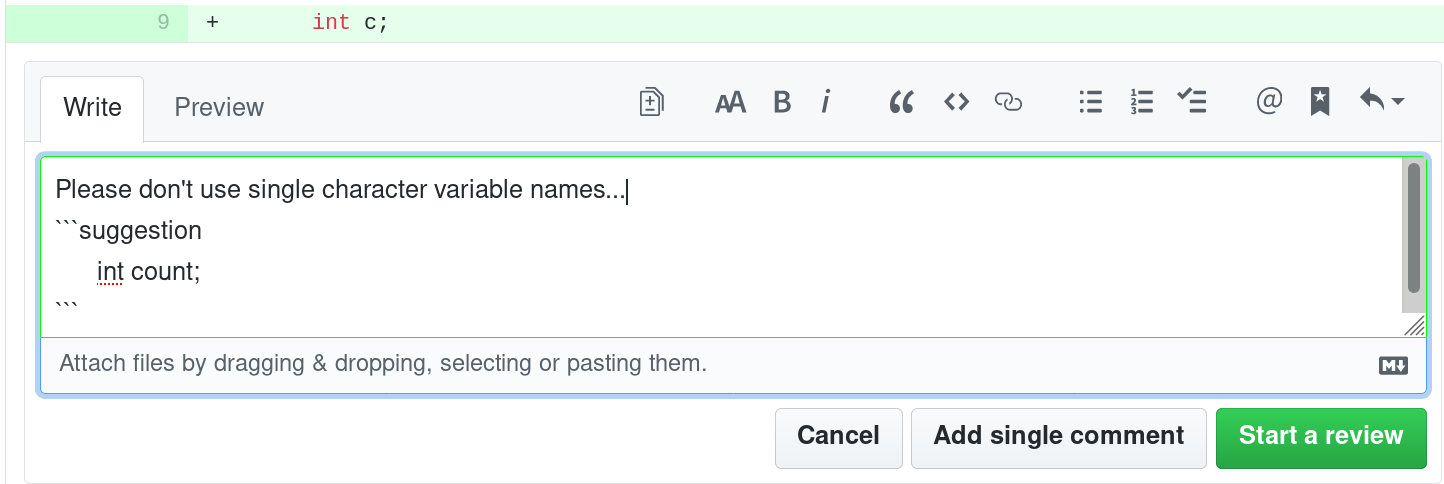
\includegraphics[width=\textwidth]{images/sugg2.png}
   (c) Developer applies suggestion from reviewer \\
    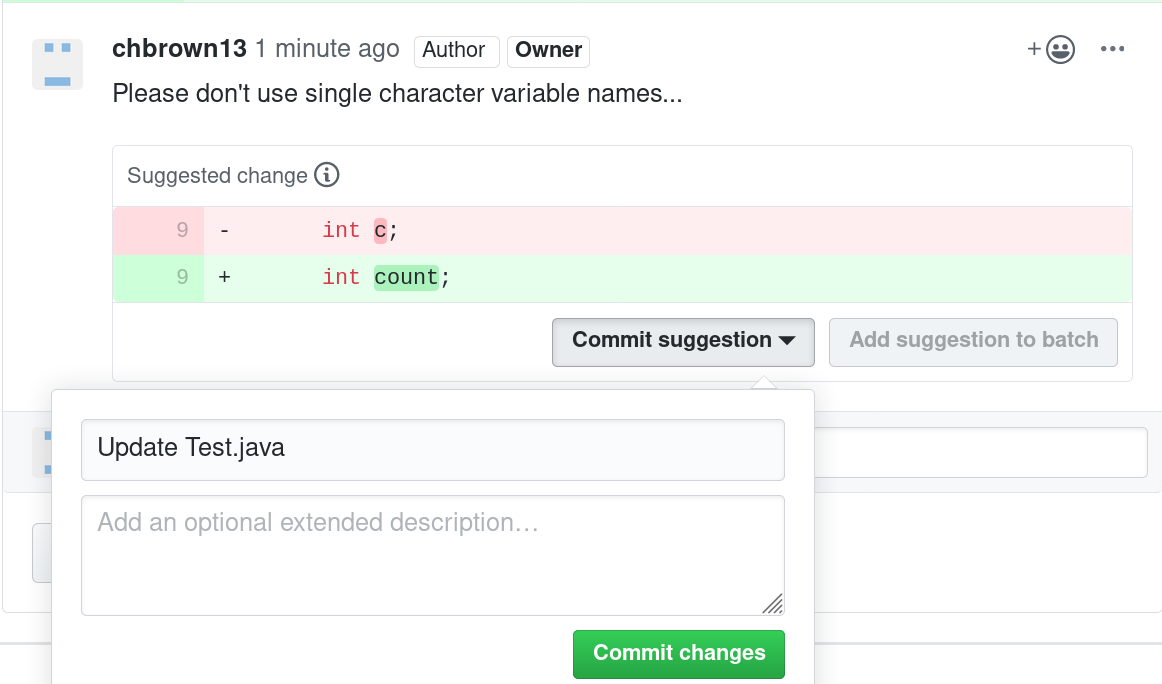
\includegraphics[width=\textwidth]{images/sugg3.png}
    \caption{GitHub Suggested Changes Example}    
    \label{fig:sugg} 
\end{figure}

\subsubsection{Research Questions:}

\begin{itemize}
    \item[\textbf{RQ1}] What suggestions do developers make with suggested changes?
    \item[\textbf{RQ2}] How effective is the suggested changes feature on GitHub?
    \item[\textbf{RQ3}] How useful is the suggested changes feature for developers?
    \item[\textbf{RQ4}] How well does the suggested changes feature generalize to other types of recommendations?
\end{itemize}

\subsubsection{Proposed Methodology:} For this research, we plan to conduct a multimethodology study divided into two phases to gather and analyze data to answer each of our research questions. \\

\subsubsection{Phase 1: \textit{An Empirical Study on GitHub Suggested Changes}} \hfill\\

The first phase of this work explores the usage and effectiveness of suggested changes on GitHub to answer the first two research questions.

\paragraph{Data Collection.}

To collect suggested changes to classify for RQ1, we developed a script to programmatically search for instances of the \sugg tag in pull request comments (See Figure~\ref{fig:sugg}b). The \sugg tag indicates that reviewer used this feature to propose a suggestion on a pull request. To gather projects and pull requests to analyze, we used the GitHub API to sort repositories by the most recently updated pull requests to compile a list of pull request with suggested changes. The script for automatically detecting uses of the suggested changes feature on GitHub pull requests is publicly available online.\footnote{\url{https://github.com/chbrown13/suggestions}}

To explore the effectiveness suggested changes, pull requests, and issues for recommendations to developers on GitHub, we mined GitHub repositories to analyze these systems. We collected pull requests and issues on the top-forked projects that have PRs with suggested changes. We analyzed the repositories with the most forks because GitHub recommends forking projects to create pull requests,\footnote{\url{https://help.github.com/en/articles/fork-a-repo}} and suggested changes require PRs to make recommendations. Additionally, our we  limited our dataset to activity after October 2018 when the suggested changes feature was introduced. To answer RQ2, we analyzed a total of 3683 suggested changes from 11869 pull request review comments, 3882 pull requests, and 3516 issues. We used two metrics to measure the effectiveness of each system: \textit{acceptance} and \textit{timing}. A list of projects used for this evaluation is available in Table~\ref{tab:projects}. 

\paragraph{Classifying types of suggested changes.}
To categorize the types of changes developers suggest with this feature, we randomly sampled 100 recently updated pull requests with an instance of the \sugg tag in the comments. A random sample was used to avoid bias from classifying suggested changes from the same GitHub users and projects. To identify categories of suggested changes, two researchers performed an \textit{open} coding by analyzing pull requests review comments with the \sugg tag and code changes recommended by developers with this feature (inter-rater agreement = 71\%, Cohen's $\kappa$ = 0.5942). The two coders then came together to discuss their results come to an agreement. Below we define and provide examples of the four identified categories for suggested changes:

\textbf{Corrective:} The corrective category refers to using suggested changes to fix issues found in the code. Software engineering research shows corrective changes are important for improving code quality. For example, Bacchelli and colleagues found that finding defects is the primary motivation for software engineers to conduct code reviews~\cite{bacchelli2013codereview}. For example, Figure~\ref{fig:categories}a presents a corrective suggested change from a reviewer on a developer's pull request. The suggestee referred to a variable as a global variable instead of a class variable, and the suggester proposes a fix by adding the \texttt{self} keyword.\footnote{\url{https://github.com/zeit/next.js/pull/7696\#discussion_r302333269}}

\textbf{Improvement:} Improvement suggested changes refer to when reviewers recommend code changes to refactor or optimize a contributor's code. Developers at Microsoft reported that code improvements are the primary benefit of code reviews.\footnote{\url{https://www.michaelagreiler.com/code-reviews-at-microsoft-how-to-code-review-at-a-large-software-company/}} Additionally, further analysis by Bacchelli and colleagues revealed that, while developers reported correcting defects as the primary motivation for code reviews, code improvements were the most frequently mentioned motivation~\cite{bacchelli2013codereview}. Figure~\ref{fig:categories}b presents an instance of an improvement suggested change, where the suggester proposes improving the readability of the suggestee's code by renaming a variable from \texttt{x} to \texttt{manifest}.\footnote{\url{https://github.com/gatsbyjs/gatsby/pull/13471\#discussion_r277948539}}

\textbf{Formatting:} The formatting category refers to refactoring code changes that impact the style and presentation of the code. Fixing formatting issues is also an important change to improve code. Bacchelli and colleagues reported developers also found code reviews to be useful for ensuring code styles and standards are consistent between programmers on development teams~\cite{bacchelli2013codereview}. An example of a formatting suggestion is presented in Figure~\ref{fig:categories}c.\footnote{\url{https://github.com/numba/numba/pull/4204\#discussion_r310598073}} where the suggester recommends changes to fix spacing issues in the suggester's code that violate the Python PEP8 whitespace standards.\footnote{\url{https://www.python.org/dev/peps/pep-0008/\#whitespace-in-expressions-and-statements}}

\textbf{Non-Functional:} Non-functional suggested changes refer to modifications reviewers recommend outside of the code. This includes suggestions to fix spelling and grammar issues or reword phrases in code documentation and comments. Non-functional changes are prevalent in software engineering, for example Beller and colleagues found that documentation changes are the most frequent type of fixes applied during code reviews for open source software~\cite{beller2014modern}. Figure~\ref{fig:categories}d presents an example of a non-functional suggested change. In this case, the suggester discovers a typo where the suggestee misspelled \textit{deserialize} in a documentation files and uses the suggested changes feature to recommend a fix for the error.\footnote{\url{https://github.com/microsoft/terminal/pull/1258\#discussion_r293932790}}

\begin{figure}[]
\centering
    \textbf{(a) Corrective: \\}
    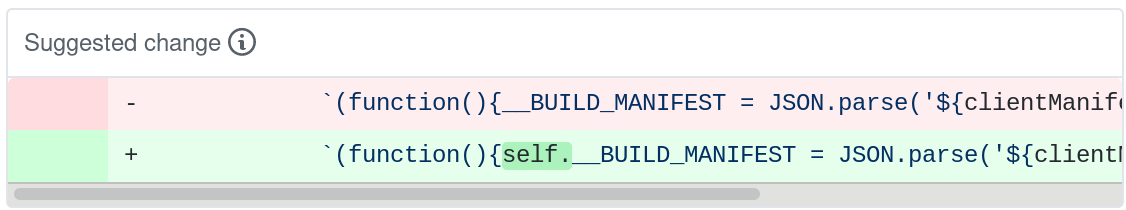
\includegraphics[width=\textwidth]{images/correct.png}
    \textbf{(b) Improvement: \\}
    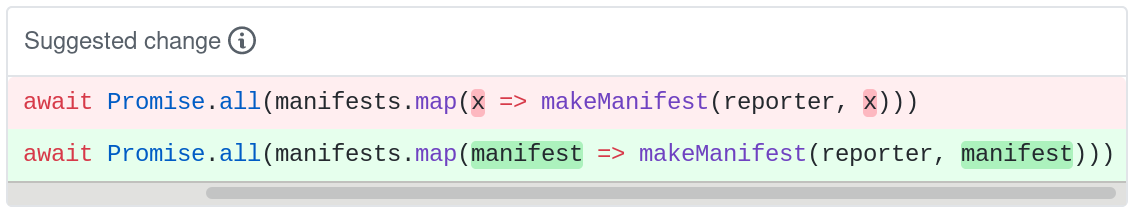
\includegraphics[width=\textwidth]{images/improve.png}
    \textbf{(c) Formatting: \\}
    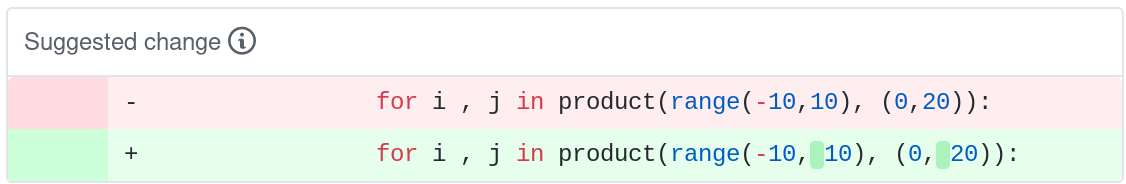
\includegraphics[width=\textwidth]{images/format.png}
    \textbf{(d) Non-Functional: \\}
    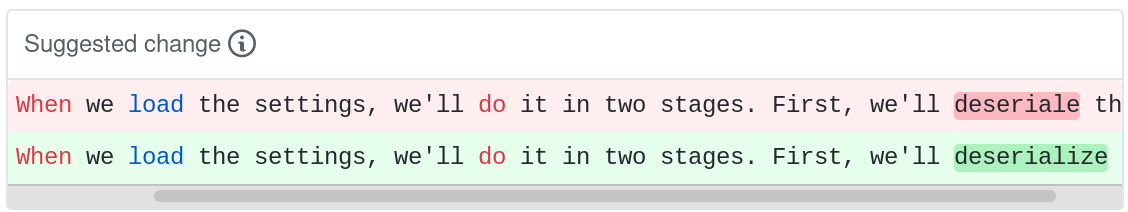
\includegraphics[width=\textwidth]{images/nonfunc.png}
    \caption{Suggested Changes Categories}    
    \label{fig:categories} 
\end{figure}

\paragraph{Determining acceptance of recommendations.}

We define acceptance as the process of users welcoming suggested changes recommended by another developer. Accepting these suggestions indicates an effective recommendation because the author trusts changes and believes it will be beneficial to the code. Research shows this concept is important in software development. For example, to emphasize the importance of acceptance in software engineering, Middleton and colleagues argue receiving code contributions from outside developers is essential for the maintenance and evolution of open source software~\cite{Middleton2018Contributions}.

Since the suggested changes feature is currently not supported by the GitHub API,\footnote{\url{https://github.community/t5/GitHub-API-Development-and/Accessing-the-new-quot-GitHub-Suggestions-quot-via-API-public/td-p/13922}} we extended the suggested changes detection script to examine commits made on pull requests with suggestions. To determine whether suggestions were accepted or rejected, our script found instances of pull requests with suggested changes. Then, it parsed review comments on the PR to extract the recommended code modifications between the \sugg tag and the ending \texttt{'''}. Finally, it checked whether the suggested line of code was present in another commit after the comment was made to the pull requests on the same file that received the suggested change. Suggested changes with lines of code that were found to be integrated in a subsequent commit on a pull request were considered accepted, otherwise they were regarded as rejected.

To determine the acceptance of pull requests, we simply used the existing GitHub status. In the pull-based software development model, accepted changes must be merged into the source code~\cite{gousios2014pullrequests}. In this case, a Merged PR is considered accepted because the recommended code changes were reviewed and approved by a maintainer to be integrated into the project. For issues, the only possible statuses are Open or Closed. Thus, we were not able to automatically detect if recommendations from this system were closed to be accepted into repositories or closed to be ignored. To analyze only accepted issues with recommendations, we filtered out issues with GitHub labels \texttt{bug} and \texttt{duplicate} to avoid bug reports and multiple instances of the same issue.\footnote{\url{https://help.github.com/en/articles/about-labels}} After automatically filtering these labels, a researcher manually examined the title, description, discussion, and status of issues to code issues based on two criteria: 1) if they contain a \textit{recommendation} or \textit{no recommendation} and 2) if the recommendation was \textit{accepted} or \textit{not accepted} into the project. Accepted issues are those with recommendations that are integrated with a pull request or commit to the repository.

\paragraph{Determining timing of recommendations.}

The second metric used to determine the effectiveness of recommendations was the amount of time developers took to accept a suggestion, or acceptance time, for each system. In behavioral economics, Kocher and colleagues suggest the time to make decisions is important to the quality of choices because ``time \textit{is} money"~\cite{kocher2006time}. In software engineering, research also shows that time can impact the cost and effort required to fix bugs in code~\cite{Williams2007FaultFixTime}. To measure timing for each system, we calculated the amount of time between the creation of the recommendation and its acceptance into the repository.

For suggested changes, we measured the acceptance time as the amount of time between a reviewer commenting on a pull request with the \sugg tag until the time a subsequent commit adding the suggested line of code was created on the pull request. To measure the acceptance time for pull requests, we used the GitHub API to calculate the difference between the time from when a GitHub developer creates a pull request and when the pull request is merged into the repository by a project maintainer. After manually inspecting issues to determine they have an accepted recommendation, we used the GitHub API to determine the acceptance time for these issues by calculating the difference between the time the issue was created and the time it was closed.

\begin{table}[tbh]
\centering
\begin{tabular}{ lllrrr } \hline
  \textbf{Project} & \textbf{Language} & \textbf{Forks} & \textbf{Suggestions} & \textbf{PRs} & \textbf{Issues} \\ \hline
 qmk/qmk\_firmware & C & 8723 & 3627 & 1997 & 290 \\
 h5bp/Front-end-Developer-Interview-Questions & HTML & 8325 & 1 & 35 & 5  \\
 Azure/azure-quickstart-templates & PowerShell & 7743 & 2 & 921 & 147 \\
 firebase/quickstart-android & Java & 5603 & 2 & 91 & 124 \\ 
 mavlink/qgroundcontrol & C++ & 1584 & 4 & 402 & 267 \\
 qgis/QGIS & C++ & 1516 & 47 & 436 & 2683 \\

\end{tabular}
\caption{RQ2 Study Projects}
\label{tab:projects}
\end{table}

\subsubsection{Phase 2: \textit{Developer Feedback on Suggested Changes}}

The second phase consisted of a survey and user study to answer the last two research questions on the usefulness and generalizability of GitHub suggested changes.

\paragraph{Data Collection.}

To determine the usefulness of suggested changes, we surveyed developers who interacted with the feature on GitHub. Surveys were emailed to users with publicly available email addresses who either received or made a suggestion on a pull request within the last six months. Our survey asked users how useful they found the this feature using a 5-point Likert scale as well as free response questions to provide details on what specifically they find useful or not useful about the system and how it is integrated it into their project.

To answer RQ4, we conducted a user study to examine applying the suggested changes feature to tool recommendations. We recruited 14 professional software developers, presented in Table~\ref{tab:participants}, to participate in this study. The participants averaged 5 years of industry experience in various roles such as Software Engineer, Software Developer, Quality Engineer, Consultant, Data Migration Consultant, Support Specialist, User Researcher, and Technical Test Lead. Additionally, all participants were at least somewhat familiar with GitHub. We conducted a think aloud study with a semi-structured interview and audio and screen recorded all sessions to collect feedback from developers on how well the suggested changes feature translates to software engineering tool recommendations. 

\paragraph{Determining usefulness of suggestions.}

We emailed surveys to a total of 570 GitHub users who interacted with suggested changes and received 39 responses (7\% response rate).  Throughout the remainder of this paper, we use the \see- prefix to describe a \textit{suggestee}, or a contributor who received a suggested change on their pull request, and the \ser- prefix to indicate a \textit{suggester}, or a reviewer who made a comment with the suggested changes feature on a pull request. We aggregated the Likert scores to examine the overall usefulness, then two experts \textit{open} coded the open-ended responses from developers on the useful (72\%, $\kappa$ = 0.6828) and unuseful (77\%, $\kappa$ = 0.7125) aspects of suggested changes. The researchers discussed derived categories and came to a consensus on themes found in comments. To resolve disagreements in coding statements, the first author acted as the tie-breaker. The primary inconsistencies in coding came from determining the existence of multiple themes since responses from developers could span more than one category.

\paragraph{Determining the generalizability of recommendations.}


To determine the impact of suggested changes on tool recommendations, we asked participants to interact with sample recommendations from a suggested change, pull request, issue, and email. Participants were asked to provide a Likert-scale ranking on how likely they would adopt the tool and to discuss what they like and dislike about each system as well as provide insight into what makes tool recommendations effective in general. Figure~\ref{fig:tool} presents an example of the prototype suggested change recommendation system, using the feature to suggest a fix for a bug reported by static analysis output and recommend a tool for developers to find and prevent errors in the future. Staged recommendations for pull requests, issues, and emails contained similar text suggesting tools to participants from each system. To analyze feedback on this design, we aggregated the Likert scores and open-ended feedback from participants. For the rest of this paper, user study participants are indicated with a P-prefix. We transcribed and analyzed recordings of sessions to present feedback from developers on receiving tool recommendations with suggested changes.

\begin{table*}[]
\centering
\begin{tabular}{ lrlll } \hline
  \textbf{ID} & \textbf{Experience (yrs)} & \textbf{GitHub Familiarity} & \textbf{OSS Contributions} & \textbf{Tool Usage} \\ \hline
 % P0.1 & PhD student & 3 & Moderate & Very Frequently \\  
 % P0.2 & PhD student & 0.5 & Moderate & Rarely \\ 
 P1 & 30 & Very Familiar & Occasionally & Very Frequently \\  
 P2 & Less than 1 & Moderately Familiar & Never & Never \\ 
 P3 & Less than 1 & Very Familiar & Rarely & Moderately Frequent \\  
 P4 & 8 & Very Familiar & Very Frequently & Very Frequently \\ 
 P5 & 10 & Familiar & Rarely & Moderately Frequent \\
 P6 & 5 & Moderately Familiar & Occasionally & Very Frequently \\
 P7 & 6 & Familiar & Frequently & Very Frequently \\
 P8 & 6 & Familiar & Very Frequently & Very Frequently \\
 P9 & Less than 1 & Moderately Familiar & Occasionally & Very Frequently \\
 P10 & 1 & Moderately Familiar & Occasionally & Very Frequently \\
 P11 & 3 & Familiar & Very Frequently & Very Frequently \\
 P12 & 3 & Familiar & Rarely & Very Frequently \\
 P13 & 1 & Moderately Familiar & Never & Never \\
 P14 & 1 & Moderately Familiar & Never & Frequently \\
 \hline
 
\end{tabular}
\caption{RQ4 User Study Participants}
\label{tab:participants}
\end{table*}

\begin{figure}[]
	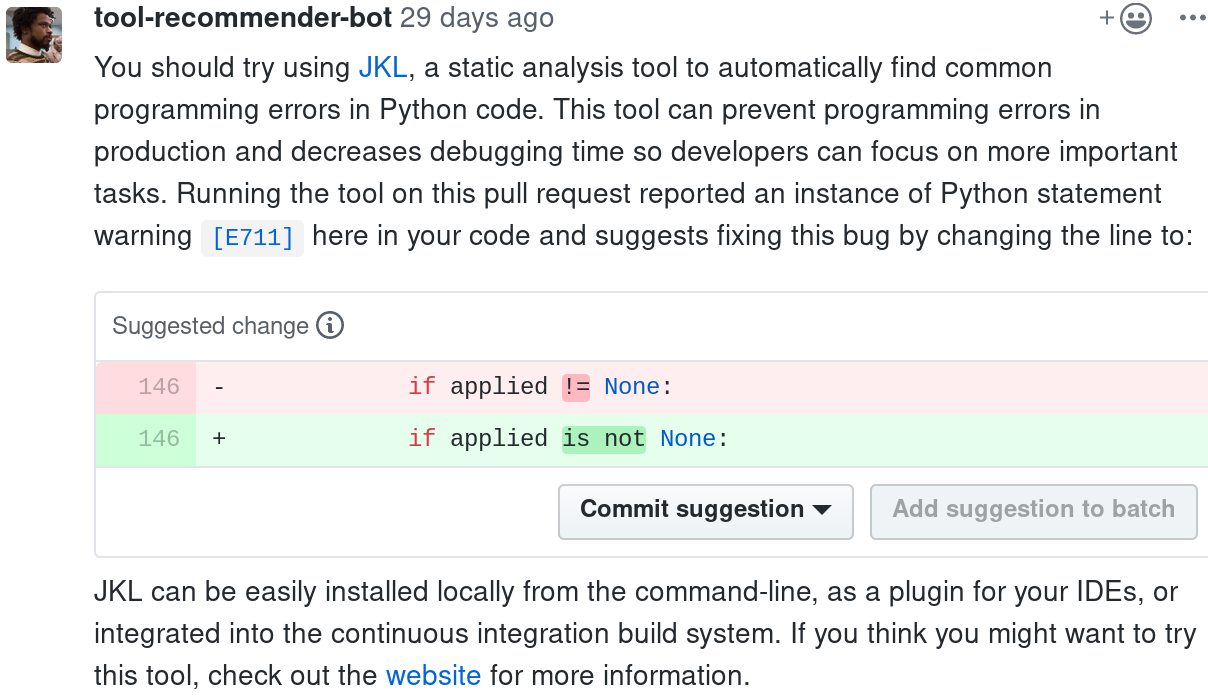
\includegraphics[width=\textwidth]{images/auto_suggest.png}
	\caption{Mock Recommender system with suggested changes}	
	\label{fig:tool} 
\end{figure}


\subsubsection{Expected Results:} From this evaluation, I expect to gain insight into the GitHub suggested changes feature. For RQ1, we hypothesize that suggested changes are useful for recommending a wide variety of code changes. For RQ2, we hypothesize suggested changes are as effective as other systems for recommendations between users on GitHub. For RQ3, we expect users find this new feature very useful for suggesting and receiving code change recommendations. Finally, for RQ4 we believe the design of this system can generalize to other types of recommendations and is preferred by software developers for recommending static analysis tools. Overall, we expect the results from this study to motivate the use of digital nudges for making effective recommendations to developers. The results of this evaluation were submitted for publication to the 2020 International Conference on Software Engineering (ICSE 2020).\footnote{\url{https://conf.researchr.org/home/icse-2020}}

% \paragraph{RQ1: Usage.}

% \begin{table}[H]
% \centering
% \begin{tabular}{ |c|c|c|} \hline
%   & \textbf{\textit{n}} & \textbf{Percentage} \\ \hline
%  Non-Functional &  36 & 36\% \\ \hline
%  Improvement & 34  & 34\% \\ \hline 
%  Corrective &  16 & 16\% \\ \hline
%  Formatting & 14 & 14\% \\ \hline
% \end{tabular}
% \caption{Suggested Change Categories}
% \label{tab:rq1}
% \end{table}

% We discovered that most suggested changes to developers were recommendations for non-functional changes. Table~\ref{tab:rq1} presents our findings for each category from 100 randomly sampled uses of the suggested changes feature on GitHub. While non-functional changes were the most frequent type of changes recommended with this feature, we found that suggested changes are also useful for recommending a wide variety of code modifications to developers during reviews. 

% \paragraph{RQ2: Effectiveness.}

% Our results suggest that pull requests are still the primary method for GitHub developers to accept recommendations. Table~\ref{tab:accept} presents our results for acceptance for each system. Using a chi-square test to analyze the outcome of recommendations for each group, we found that the difference in acceptance was statistically significant for suggested changes, pull requests, and issues ($\chi^2$ = 1128.7155, p < .00001, $\alpha$ = .05). Approximately 78\% of PRs we analyzed were merged into repositories compared to 69\% of suggested changes and only 17\% of issues. While suggested changes are a relatively new feature, many projects have already adopted the pull-based model for software development on GitHub~\cite{gousios2014exploratory,  gousios2015work}.

% \begin{table}[H]
% \centering
% \begin{tabular}{ |c|c|c|} \hline
%   & \textbf{\textit{n}} & \textbf{Rate} \\ \hline
%  suggestions & 2554 & 69.3\% \\ \hline 
%  pull requests & 3044 & 78.4\% \\ \hline
%  issues & 133 & 17.2\% \\ \hline
% \end{tabular}
% \caption{Acceptance Rate}
% \label{tab:accept}
% \end{table}

% For timing, we found that recommendations for suggested changes are accepted into repositories almost twice as fast as pull requests, while issues remain much less effective. Table~\ref{tab:time} presents the average acceptance time for each type of recommendation. Using the Kruskal-Wallis test to analyze the time data, we found a significant difference in the amount of time taken to accept a recommendation for each system (Kruskal-Wallis = 391.844102, \textit{p} < .0001, $\alpha$ = .05). This indicates that developers are able to make a decision on whether to accept or reject recommendations using suggested changes much faster than with pull requests or issues. Shorter acceptance times are useful in software engineering to help reduce \textit{fault fix latency}, or the amount of time a defect exists in code~\cite{Layman2007FaultFixTime}. This can prevent wasted time, effort, and costs to fix latent bugs during the software development process.

% \begin{table}[H]
% \centering
% \begin{tabular}{ |c|c|c|c| } \hline
%   & \textbf{Average (days)} & \textbf{Median (days)} \\ \hline
%  suggestions & 2.9 & 0.3 \\ \hline 
%  pull requests & 5.0 & 0.8 \\ \hline
%  issues & 28.5 & 2.6 \\ \hline
% \end{tabular}
% \caption{Acceptance Time}
% \label{tab:time}
% \end{table}

% To further understand the impact of suggested changes, we observed their impact on the effectiveness of pull requests themselves. We collected results on the acceptance and timing of pull requests with and without suggestions. The findings from this analysis are presented in Table~\ref{tab:acceptPR}. We found that that pull requests with suggested changes were accepted significantly more often than pull requests without them ($\chi^2$ = 6.1296, \textit{p} = 0.013294, $\alpha$ = .05). However, we also surprisingly discovered that pull requests with suggested changes take significantly longer to be accepted than those without (Wilcoxon, \textit{p} < .0001, $\alpha$ = .05). This may be due to the fact that, while individual suggested changes are quickly accepted by developers, one pull request often has multiple changes suggested. In the data collected study the influence of suggested changes on PRs, we observed each pull request had an average of six comments with suggested changes. This shows that pull requests with suggested changes are more complex. While this feature helps resolve problems in code reviews and eventually get pull requests accepted, they also add more time to code inspections.

% \begin{table}[H]
% \centering
% \begin{tabular}{ |c|c|c|c| } \hline
%   \textbf{Pull Requests} & \textbf{\textit{n}} & \textbf{Acceptance} & \textbf{Timing (days)} \\ \hline
%  with suggestions & 559 & 79.8\% & 8.88 \\ \hline 
%  without suggestions & 3323 & 78.2\% & 4.34 \\ \hline
% \end{tabular}
% \caption{Pull Request Data}
% \label{tab:acceptPR}
% \end{table}

% \paragraph{RQ3: Usefulness.}

% Figure~\ref{fig:usefulness} presents the Likert results on how useful the 39 survey respondents found the suggested changes feature. No GitHub users who interacted with this feature responded that it was Not at All Useful. Meanwhile, 95\% of suggestees and 76\% of suggesters responded they believe the suggested changes feature is Useful or Very Useful. This suggests that GitHub users find this system useful for both receiving recommendations from peers as well as sharing knowledge and making suggestions to colleagues on GitHub.

% \begin{figure}
% \begin{tikzpicture}
% \begin{axis}[
%     xbar stacked,
%     ytick=data,
%     axis y line*=none,
%     axis x line*=bottom,
%     tick label style={font=\footnotesize},
%     legend style={font=\footnotesize},
%     label style={font=\footnotesize},
%     xtick={0,5,10,15,20,25},
%     width=\textwidth,
%     bar width=6mm,
%     xlabel= Number of Participants,
%     yticklabels={Not at All Useful, Somewhat Useful, Moderately Useful, Useful, Very Useful},
%     xmin=0,
%     xmax=25,
%     area legend,
%     y=8mm,
%     enlarge y limits={abs=0.625},
% ]
% % Suggesters
% \addplot[fill=lightgray] coordinates
% {(0,0) (1,1) (3,2) (7,3) (6,4)};
% % Suggestees
% \addplot[fill=black] coordinates
% {(0,0) (0,1) (1,2) (14,3) (7,4)};
% \legend{Suggester, Suggestee}
% \end{axis}  
% \end{tikzpicture}
% \caption{Survey Results}
% \label{fig:usefulness}
% \end{figure}

% To further examine the usefulness of suggested changes, we asked survey participants to provide open-ended responses describing what they find useful or not useful about this feature. Table~\ref{tab:useful} presents the number of comments observed in feedback derived from developers. A large majority of feedback from programmers consisted of complaints about desired features currently not supported by GitHub suggested changes. We combined comments that refer to functionality out of scope for suggested changes, such as multi-line suggestions and squashing commits, as \textit{unsupported features}. We found the inability to support advanced features weighed on participants' overall perceived value of the feature. For example, \ser11, who ranked the suggested changes feature as Somewhat Useful, responded they desired a ```force push' option, because that matches our workflow". For feedback on the current implementation of the suggested changes feature, 15 developers found it inconvenient to integrate this system with their existing tools and processes. For instance, \see16 complained `their `CI process doesn't work on suggested change[s]".

% The main feedback we discovered on the usefulness of suggested changes is that they are effective for communication between developers. This category refers to the understanding and clarity in transferring knowledge between peers, and 17 comments mentioned this feature allowed developers to share and understand feedback clearly during code reviews. For example, \ser12 responded ``I find it *so* useful. It completely removes all ambiguity about what I'm asking for". Another key benefit of suggested changes is the timing of this feature, with 11 participants noting it ``accelerates getting pull requests accepted" (\see4) and ``speeds up the review process" (\see18). While programmers applauded the clarity and speed of suggested changes and disapproved of their lacking functionality and poor integration, they had mixed consensus on the actionability and conciseness of this feature. 


% \begin{table}[H]
% \centering
% \begin{tabular}{ |c|c| } \hline
%  \textbf{Useful} & \textbf{\textit{n}} \\ \hline
%  Communication & 17 \\ \hline
%  Conciseness & 13 \\ \hline 
%  Timing & 11 \\ \hline
%  Ease of Use & 7 \\ \hline
%  Actionability & 6 \\ \hline
%  Location & 5 \\ \hline
%  Scalability & 4 \\ \hline
%  Did Not Answer & 4 \\ \hline
%  Code & 3 \\ \hline
%  Attribution & 1 \\ \hline
% \end{tabular}
% \begin{tabular}{ |c|c| } \hline
%  \textbf{Unuseful} & \textbf{\textit{n}} \\ \hline
%  Unsupported Features & 24 \\ \hline 
%  Integration & 15 \\ \hline
%  Actionability & 12 \\ \hline
%  Conciseness & 6 \\ \hline
%  Formatting & 4 \\ \hline
%  Did Not Answer & 3 \\ \hline
%  Nothing & 3 \\ \hline
%  Mentoring & 1 \\ \hline
%  Rejection & 1\\ \hline
%   & \\ \hline
% \end{tabular}
% \caption{Number of Comments for Feedback Categories}
% \label{tab:useful}
% \end{table}

% \paragraph{RQ4: Generalizability.}

% Based on the results from the user study, we found that the suggested changes feature was the preferred tool recommendation method by developers who participated in our study. Table~\ref{tab:rank} shows the average and median Likert scores representing the likelihood participants would adopt the tool from each method of recommendation. The Kruskal-Wallis test was used to statistically measure differences in developer responses to tool recommendations from suggested changes, pull requests, issues, and email. We found a significant difference in likelihood of adoption provided by participants for the four systems for recommendations (Kruskal-Wallis, \textit{p} = .00079, $\alpha$ = .05). This shows that the design of the suggested changes feature is not only useful for suggesting code modifications during code reviews, but can also apply to software engineering tool recommendations to developers.

% \begin{table}[H]
% \centering
% \begin{tabular}{ |c|c|c| } \hline
%   & \textit{\textbf{Average Score}} & \textit{\textbf{Median}} \\ \hline
%  Suggestions & 4 & 4 \\ \hline 
%  Pull Requests & 3.71 & 4 \\ \hline 
%  Issues & 2.86 & 3 \\ \hline 
%  Email & 2.36 & 2 \\ \hline 
% \end{tabular}
% \caption{Effectiveness for Developers}
% \label{tab:rank}
% \end{table}

% The user study also consisted of a semi-structured interview, where we were particularly interested in gaining insight into using suggested changes for suggesting tools and improving developer recommendations. We used this feedback as well as developer survey responses on the usefulness of suggested changes to motivate the four design principles for overcoming barriers to peer interactions and improving automated recommendations to software developers based on the suggested changes feature: \textit{social recommendations}, \textit{user-driven communication}, \textit{actionable recommendations}, and \textit{receptive choice architecture}. The results of this study have been submitted for publication at the 2020 International Conference on Software Engineering (ICSE).


\subsection{[\nudgeT] ``Nudging Students Toward Better Software Engineering Behaviors" (Proposed, Spring 2020)}

\subsubsection{Motivation:}

To integrate user receptiveness~\cite{VLHCC} and improve on the effectiveness of a naive bot~\cite{BotSE} for making suggestions to improve developer behavior, we propose implementing a new bot to nudge software engineers to adopt developer behaviors. To understand the impact of implementing automated recommendations as digital nudges, we plan to implement and evaluate a novel recommendation approach in a new system: \TOOL. While \tool and the \tele approach failed to effectively recommend static analysis tools to developers, we aim to enhance \TOOL by incorporating our conceptual framework for designing effective developer recommendations in addition to design implications from the results of the \sugg study examining an existing system that can be considered a digital nudge. To evaluate this system, we plan to examine how recommendations from \TOOL improve the decision-making and behavior of students in a college-level software engineering course. While research shows that automation is useful to help with grading and teaching in introductory computer science courses~\cite{singh2013automated} and providing feedback to students~\cite{hu2019feedback}, there is little to no work exploring the use of automated recommendations to improve student behavior. We aim to show that this new system can improve student behavior in software engineering education and the results from this evaluation can provide implications for making effective recommendations to improve the behavior of software engineers in industry.

\subsubsection{Software Engineering Education:} Research suggests improvements are needed for software engineering education and the future of the software industry. The ACM notes that there is a ``crisis" in Computer Science Education that will result in necessary computing-related jobs going unfilled~\cite{emptyfailure}. Furthermore, even though the computer science major is one of the most popular fields of study at universities, it also has a very high attrition and failure rate~\cite{beaubouef2005high}. For software engineering education, a subset of computer science, researchers have explored problems with effectively preparing students for industry. Jazayeri outlines challenges of teaching software engineering and provides ideas for a new curriculum and skills to educate successful software engineers~\cite{jazayeri2004education}. Furthermore, Devadiga argues that topics taught in school are often unrelated to industry practice and suggests merging with startups to improve SE education~\cite{devadiga2017software}. Additionally, Heckman and colleagues present ``the good, the bad, and the ugly" of teaching software engineering to students using an open source software system~\cite{Heckman2018Itrust}. Several issues they found include delayed feedback, group dynamics, high workload, and aggressive scheduling. We aim to improve on these problems in software engineering education by using nudges to encourage students to adopt useful developer behaviors.

\subsubsection{Research Questions:}

\begin{itemize}
    \item[\textbf{RQ1}] How do nudges influence software engineering student productivity?
    \item[\textbf{RQ2}] How do nudges impact the quality of software engineering student projects?
\end{itemize}

\subsubsection{Proposed Methodology:}

To evaluate integrating nudge theory into developer recommendations, we plan to conduct a mixed-methods research study.

\paragraph{Data Collection.} The data for this evaluation will be collected from the undergraduate (CSC 326) Software Engineering course at North Carolina State University. The final project for the course will require students to maintain and add new features to iTrust\footnote{\url{https://github.ncsu.edu/engr-csc326-staff/iTrust2-v5}}, an electronic health records system. First, we will analyze data by mining team GitHub repos for final projects from previous semesters of CSC 326. This will help us determine which project milestones to nudge for as well as when to nudge. During this stage, we will collect information from iTrust repositories and past teams such as overall project grade, submission times, total number of commits, amount of time to complete various milestones, and code contributions by each group member. While the project requirements change for the team project each semester, each iteration of the class will have similar milestones to complete every year. Additionally, we plan to conduct to pilot and test \TOOL this semester on a project for the graduate software engineering course (CSC 510).

After examining projects from prior semesters to determine the best behaviors and timing for nudges, we plan to mine repositories for the CSC 326 final project in Spring 2020 to answer our research questions. Participants will be volunteer software engineering groups from the class who opt-in to receiving notifications from a bot and consent to using the data collected for this research. We plan to gather quantitative data based on student behaviors and performance while developing their iTrust project based on recommendations from \TOOL. Additionally, we plan collect qualitative data by surveying students to gather feedback and learn about their perception of nudges from our automated system.

\paragraph{Implementing \TOOL.} To build our new \TOOL recommender system, we utilize the GitHub API to mine repositories and track behaviors of students. This system will implement several different types of interventions to encourage students to adopt better behaviors based on monitored activity. We plan to design our bot to incorporate results from the prior work to address our conceptual framework for making effective recommendations to developers. In our evaluation, \TOOL will send notifications to students encouraging them to adopt better software development behaviors for their project. The input to the system will be a YAML configuration file mapping project milestones with deadlines and containing other information such as project team members and contact information. \TOOL will be deployed on Jenkins servers used for the CSC 326 course. Our goal is for software engineering educators to be able to customize \TOOL and integrate it into their SE courses and projects, and for software engineering researchers to be able to extend this system to recommend useful behaviors to professional developers contributing to software applications. The code for \TOOL will also be open sourced and publicly available online.\footnote{\url{https://github.com/chbrown13/nudge-bot}}

\paragraph{Defining student behaviors.} To answer RQ1, we will observe the impact of nudges on influence software engineering student project management behaviors. We aim to show that nudging students to adopt useful project management behaviors can improve the quality of their project and development productivity.

\textbf{Project Management:} Poor project management is a problem that negatively impacts software engineering students Beaubouef and colleagues note that poor project management is a hindrance for computer science students and leads to poor performance in programming classes and high attrition among CS majors~\cite{beaubouef2005high}. Additionally, this is a problem that also applies to professional software engineers in industry. Charrette argues that billions of dollars are wasted every year due to failing software projects, and suggests these project fail because of poor project management factors such as inadequate project goals, inaccurate estimates, ill-defined requirements, poor communication, and sloppy development practices~\cite{charette2005software}. The increase of distributed development teams in the software engineering industry has also led to additional project management challenges in global software development, including a lack of cultural understanding, communication, managing time differences, knowledge management and transfer in teams, trust, geographical distances, and more~\cite{niazi2016challenges}. By implementing \TOOL to influence project management behaviors in students, we aim to show that our results can translate to the software engineering industry and improving the behavior of professional developers.

For the CSC326 software engineering final project, students are asked to complete a variety of requirements for the iTrust system. For example, development process requirements for the assignment include adding a project wiki page, using GitHub issues, maintaining a passing build on Jenkins, and using a \texttt{development} branch.\footnote{\url{https://pages.github.ncsu.edu/engr-csc326-staff/326-course-page/team-project/tp-process}}. Additionally, the project requires various functional requirements to add new functionality to iTrust\footnote{\url{https://pages.github.ncsu.edu/engr-csc326-staff/326-course-page/team-project/problem-stmt\#required-elements}}. For project milestones, we plan to nudge students who have not started on specific tasks with an approaching deadline to encourage them to begin. To measure project management, we will compile a list of the functional requirements implemented and process requirements met by teams by observing GitHub repositories. We hypothesize creating nudges to encourage good project management behaviors for students and will in turn help them complete more requirements as well as adopt good practices to improve the development quality and productivity for their final project.

% \textbf{Collaboration:} Another behavior we aim to improve is teamwork between team members. Williams and colleagues found that pair learning and collaboration is beneficial for software engineering education~\cite{williams2000effects}. However, enforcing student collaboration is difficult and research also shows that issues with group dynamics is a challenge in teaching software engineering~\cite{Heckman2018Itrust}. An example of this is the case where one student writes most of the code for a project where another may slack off and do very little work. This problem also exists in the software engineering. Research shows collaboration between developers is vital for software engineering~\cite{whitehead2007collaboration}. However, Agrawal and colleagues examined ``hero" projects, where 80\% of contributions are made by 20\% of developers, and found that this practice is very common in both open source and enterprise software development~\cite{Agrawal2018Hero}. To measure collaboration, we will track GitHub activity and contributions such as commits, issues, and pull requests, for each student on their respective project teams. We believe nudging students can encourage participation and collaboration by increasing contributions from under-performing individuals to their team repository.


\paragraph{Nudging student behaviors.}

Nudges will incorporate the basic content for developer recommendations (\textit{desire}, \textit{familiarity}, \textit{social context}, and \textit{developer workflow}) as well as our developer recommendation choice architectures (\textit{actionability}, \textit{feedback}, and \textit{spatial} and \textit{temporal locality}) to automatically recommend better project management behaviors to students for their final team project. To explore the impact of actionability in developer recommendations, we plan to implement \TOOL to create \textit{active} and \textit{passive} actionable nudges to students.

\textbf{Active:} Active nudges are actionable automated interventions that partially complete programming tasks for students. We plan to determine if these recommendations will encourage users to adopt better behaviors and finish development tasks. For example, the GitHub Projects\footnote{\url{https://help.github.com/en/github/managing-your-work-on-github/about-project-boards}} is a useful feature for users to organize and track progress of their work using a project board. Tasks are created as cards and moved between columns on the board to indicate the status and track progress for each card. To encourage projects with GitHub Project boards to be active in completing tasks, an example active nudge is to automatically create cards with requirements for students to complete for their team project on their repositories. By doing this, we aim to increase awareness for students about this feature and encourage them to use project boards and cards to improve their project management activities. Overall, we hypothesize active nudges will effectively encourage software engineering students to adopt behaviors to improve project management and collaboration.

\textbf{Passive:} Passive nudges will be automated notifications that encourage students to adopt improved behaviors without impacting the project. These will be actionable visual indicators to recommend developer behaviors that would be useful to improve their project without automatically completing tasks for students. For instance, a passive nudge to encourage students to move tasks on a GitHub Projects board is to create badges to indicate their usage on a repository. Figure~\ref{fig:badges} presents an example of this, displaying a red badge to show developers are not active on their GitHub Project board (i.e. cards remain in the same column) while a green badge indicates they are active in tracking tasks on their board (i.e. cards exist and are moved between columns consistently). Research shows that badges on have been widely adopted on GitHub and repositories with this feature have a higher quality of code for the signals they indicate~\cite{trockman2018badges}. Furthermore, badges fit into the nudge theory framework by not providing incentives or preventing options for developers. Additionally, we plan to create a badge for the overall project health. This metric will indicate the likelihood a project will pass based on various factors, such as the amount of requirements completed and the recency of activities such as commits and PRs to prevent team procrastination. We hypothesize passive nudges such as these will be able to encourage students to adopt useful developer behaviors for managing project tasks and increasing team collaboration.

\begin{figure}[]
\centering
    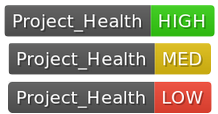
\includegraphics[width=0.3\textwidth]{images/badges.png}
    \caption{Example of Project Health badges to nudge developer behaviors}    
    \label{fig:badges} 
\end{figure}

Table~\ref{tab:nudges} presents several examples of student behaviors with potential nudges that would be implemented in our new system. The complete list of developer behavior nudges for \TOOL will be finalized after collecting data from projects from previous semesters of CSC 326, discussions with the instructors of the course for next semester, and the requirements for the final project  in Spring 2020 are officially set. More details and information about the course and milestones to complete for the team project this semester are available online.\footnote{\url{https://pages.github.ncsu.edu/engr-csc326-staff/326-course-page/team-project/}}


\begin{table}[H]
\footnotesize
\centering
\begin{tabular}{ ll } \hline
  \textbf{Behavior} & \textbf{Nudge} \\ \hline
 Manage development tasks & Badge to indicate project health (\textit{passive}) \\
 % Contribute to team project & Email students with no recent commits (\textit{passive}) \\
 Implement feature (i.e. diabetes) & Automated PR with empty class (i.e. Diabetes.java) \\
 & (\textit{active}) \\
 % Code reviews & Automated comment to review open PRs (\textit{active}) \\
\hline
\end{tabular}
\caption{Examples of nudges for software engineering students}
\label{tab:nudges}
\end{table}

\paragraph{Defining student productivity.}

To answer RQ1, we will measure student productivity using two metrics: the total amount of \textit{time} for teams to complete assignments and the amount of \textit{functional requirements} met for the team project. 

\textbf{Time:} We will examine time to discover if nudging developers impacts improves productivity and prevents procrastination on the final project. To measure time, we plan to calculate the overall amount of time needed to complete the project as well as time submitting milestones ahead of deadlines. Professional software engineers are often poor at estimating time to complete projects and fall behind schedule~\cite{charette2005software}. In SE education, Beaubouef and colleagues note that CS students often procrastinate and delay in completing tasks for their class programming assignments, which leads to lower grades and increased frustration~\cite{beaubouef2005high}. However, Willman and colleagues also found that higher performing students start and end activities earlier than their peers~\cite{willman2015study}. To encourage students to start and submit deliverables for the final CSC 326 project, we aim to nudge students to adopt better project management behaviors helping them to be more productive and finish tasks sooner.

\textbf{Functional Requirements:} Another metric for measuring productivity is to observe the number of functional processes, or technical deliverables and functionality added to iTrust for the final project. Prior work explores using function points, or the amount of functionality a system provides to users, as a metric to measure productivity~\cite{bok2000software} and predict developer effort~\cite{matson1994software}. Examples of functional requirements for the CSC 326 project this semester include adding new features such as an Oral Glucose Tolerance Test, diabetes diagnoses, and blood sugar data entry.\footnote{\url{https://pages.github.ncsu.edu/engr-csc326-staff/326-course-page/team-project/problem-stmt}} Additionally, we will observe GitHub activity for projects including commits, issues, and pull requests to measure productivity. We hypothesize that interventions from \TOOL~will encourage students to complete more functional requirements and be more productive on their final projects.

\paragraph{Defining project code quality.}

To answer RQ2, we will examine code quality by observing two metrics: \textit{grades} and \textit{process requirements}.

\textbf{Grade:} To determine if nudges impact code quality, the first metric we plan to examine is the final project grade. Figas and colleagues note that extrinsic motivators such as incentives and grades are key in motivating software engineering students to perform well on group projects~\cite{figas2013furtherance}. Additionally, Wilson and Shrock found that performance in early computer science courses can predict success in future CS classes~\cite{wilson2001contributing}. In the undergraduate software engineering course, the grading rubric for the final project consists of real-world software engineering quality metrics and process requirements, in addition to assessing the quality of the functional requirements implemented by teams on their project.\footnote{\url{https://pages.github.ncsu.edu/engr-csc326-staff/326-course-page/team-project/\#grade-categories}} We hypothesize that recommendations from \TOOL~will improve overall student grades on their final team project.

\textbf{Process Requirements:} Process requirements refer to tasks that deal with the code and development processes. Karunasekera suggests using team processes, process adherence, and quality to assess student projects to prepare software engineering students for industry careers~\cite{karunasekera2007preparing}. Additionally, software engineering industry research shows that individual programming, development team, and organizational processes are vital to the success of software engineering products~\cite{crowston2004effective}. Similarly, the CSC 326 final project requires students to follow development processes that impact code quality such as adhering to the NCSU department Java style guide,\footnote{\url{https://pages.github.ncsu.edu/engr-csc116-staff/CSC116-Materials/course-resources/style-guidelines/}} passing unit tests, at least 70\% test coverage, documenting code, conducting code reviews, adding a project wiki page and README, and maintaining passing project builds. We aim to show that both active and passive nudges to software engineering students can increase the amount of technical and team processes accomplished by development teams on their final projects.

\subsubsection{Expected Results:}

We hypothesize that active and passive nudges to software engineering students will improve their behavior while working on teams to complete a development project. Specifically, we believe that sending automated notifications to CSC 326 students from \TOOL will: 1) increase the amount of functional and process requirements implemented for development teams on the iTrust healthcare system, 2) reduce the amount of time students procrastinate and complete work on their projects, and 3) improve the overall software quality and student grades for the team project.

\newpage